\documentclass{article}[10pt]
\usepackage{multicol, enumerate, enumitem, hyperref, color, soul, setspace, parskip, fancyhdr, amssymb, amsthm, amsmath, bbm, latexsym, units, mathtools}
\everymath{\displaystyle}
\usepackage[headsep=0.5cm,headheight=0cm, left=1 in,right= 1 in,top= 1 in,bottom= 1 in]{geometry}

\begin{document}
This is the Answer Key for Module 6 Version A.

26. Which of the following equations \textit{could} be of the graph presented below?
$$  $$ 
\begin{center}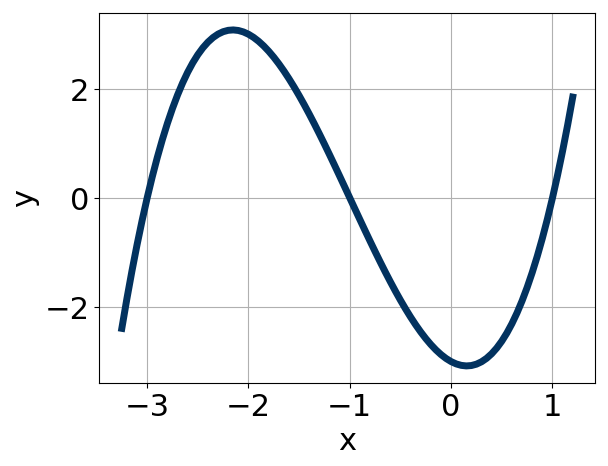
\includegraphics[scale=0.5]{../Figures/question26A.png}\end{center}The solution is $ (x + 3)(x - 1)(x + 1) $ 

\begin{enumerate}[label=\Alph*.] 
\item $ (x + 3)^2(x - 1)(x + 1) $ 

  
\item $ (x + 3)^2(x - 1)^2(x + 1) $ 

  
\item $ -(x + 3)(x - 1)(x + 1) $ 

  
\item $ -(x + 3)^2(x - 1)(x + 1) $ 

  
\item $ (x + 3)(x - 1)(x + 1) $ 

  
\end{enumerate} 
 
General Comments: Draw the x-axis to determine which zeros are touching (and so have even multiplicity) or cross (and have odd multiplicity)

-----------------------------------------------

27. Choose the end behavior of the polynomial below.
$$ f(x) = -7(x + 7)^{4}(x - 7)^{5}(x - 4)^{2}(x + 4)^{3} $$ 
The solution is  
\begin{center}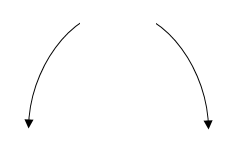
\includegraphics[scale=0.5]{../Figures/endBehaviorNegativeEven.png}\end{center}\begin{enumerate}[label=\Alph*.] 
\item Negative leading coefficient, sum of degrees is odd. 
\begin{center}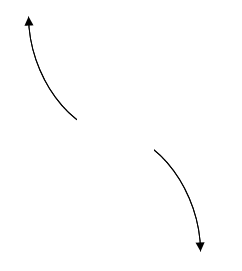
\includegraphics[scale=0.5]{../Figures/endBehaviorNegativeOdd.png}\end{center} 
 
\item Negative leading coefficient, sum of degrees is even. 
\begin{center}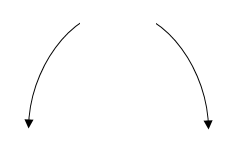
\includegraphics[scale=0.5]{../Figures/endBehaviorNegativeEven.png}\end{center} 
 
\item Positive leading coefficient, sum of degrees is even. 
\begin{center}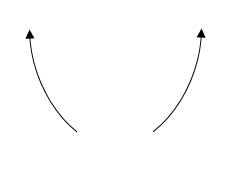
\includegraphics[scale=0.5]{../Figures/endBehaviorPositiveEven.png}\end{center} 
 
\item Positive leading coefficient, sum of degrees is odd. 
\begin{center}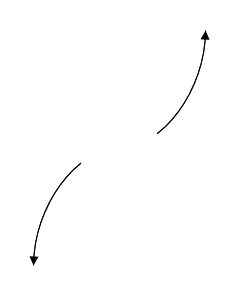
\includegraphics[scale=0.5]{../Figures/endBehaviorPositiveOdd.png}\end{center} 
 
\end{enumerate} 
 
General Comments: Remember that end behavior is determined by the leading coefficient AND the sum of the multiplicities.

-----------------------------------------------

28. Describe the zero behavior of the zero $x = -7$ of the polynomial below.
$$ f(x) = -7(x + 7)^{4}(x - 7)^{5}(x - 4)^{2}(x + 4)^{3} $$ 
The solution is  
\begin{center}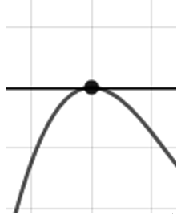
\includegraphics[scale=0.5]{../Figures/zeroBehaviorNegativeEven.png}\end{center}\begin{enumerate}[label=\Alph*.] 
\item The function is above the $x$-axis, then passes through. 
\begin{center}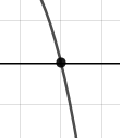
\includegraphics[scale=0.5]{../Figures/zeroBehaviorNegativeOdd.png}\end{center} 
 
\item The function is below the $x$-axis, then touches. 
\begin{center}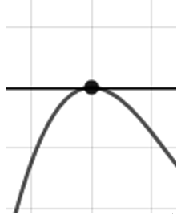
\includegraphics[scale=0.5]{../Figures/zeroBehaviorNegativeEven.png}\end{center} 
 
\item The function is above the $x$-axis, then touches. 
\begin{center}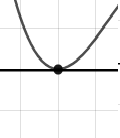
\includegraphics[scale=0.5]{../Figures/zeroBehaviorPositiveEven.png}\end{center} 
 
\item The function is below the $x$-axis, then passes through. 
\begin{center}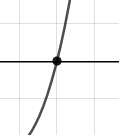
\includegraphics[scale=0.5]{../Figures/zeroBehaviorPositiveOdd.png}\end{center} 
 
\end{enumerate} 
 
General Comments: You will need to sketch the entire graph, then zoom in on the zero the question asks about.

-----------------------------------------------

29. Construct the lowest-degree polynomial given the zeros below. Then, choose the intervals that contain the coefficients of the polynomial in the form $ax^3+bx^2+cx+d$.
$$ -3, -2, \text{ and } \frac{3}{4} $$ 
The solution is $ 4 x^3 + 17 x^2 + 9 x - 18 $ 

\begin{enumerate}[label=\Alph*.] 
\item $ a \in [-2, 5], b \in [-24, -19], c \in [38, 40], \text{ and } d \in [-21, -10] $ 

  Distractor 4: This corresponds to using $(x+z_1)(x+z_2)$ for the first two terms. 
\item $ a \in [-2, 5], b \in [-22, -14], c \in [8, 12], \text{ and } d \in [14, 20] $ 

  Distractor 1: This corresponds to multiplying $(x+z_1)(x+z_2)(x+z_3)$ 
\item $ a \in [-2, 5], b \in [-10, -2], c \in [-22, -20], \text{ and } d \in [14, 20] $ 

  Distractor 3: This corresponds to using $(x+z_1)$ for the first term. 
\item $ a \in [-2, 5], b \in [12, 23], c \in [8, 12], \text{ and } d \in [-21, -10] $ 

 * This is the correct solution 
\item $ a \in [-2, 5], b \in [12, 23], c \in [8, 12], \text{ and } d \in [14, 20] $ 

  Distractor 2: This corresponds to having everything correct except the sign of the last term. 
\end{enumerate} 
 
General Comments: To construct the lowest-degree polynomial, you want to multiply out $(1x--3)(1x--2)(4x-3)$

-----------------------------------------------

30. Construct the lowest-degree polynomial given the zeros below. Then, choose the intervals that contain the coefficients of the polynomial in the form $x^3+bx^2+cx+d$.
$$ -4i \text{ and } 1 $$ 
The solution is $ x^3 - 1 x^2 + 16 x - 16 $ 

\begin{enumerate}[label=\Alph*.] 
\item $ b \in [-3.1, -0.9], c \in [15.5, 18], \text{ and } d \in [-17, -13] $ 

 * This is the correct solution 
\item $ b \in [0, 4.8], c \in [-1.2, -0.9], \text{ and } d \in [-3, 4] $ 

  Distractor 2: This distractor corresponds to using a from the complex and the other zero to make a quadratic. 
\item $ b \in [0, 4.8], c \in [-20.1, -15.9], \text{ and } d \in [11, 17] $ 

  Distractor 4: This distractor corresponds to negatives for each of the coefficients in the solution. 
\item $ b \in [0, 4.8], c \in [15.5, 18], \text{ and } d \in [11, 17] $ 

  Distractor 1: This distractor corresponds to using (x+z) for zeros. 
\item $ b \in [0, 4.8], c \in [2.1, 5.9], \text{ and } d \in [-10, -3] $ 

  Distractor 3: This distractor corresponds to using b from the complex and the other zero to make a quadratic. 
\end{enumerate} 
 
General Comments: Remember that the conjugate of $a+bi$ is $a-bi$. Since these zeros always come in pairs, we need to multiply out $(x--4i)(x+-4i)(x-1)$

-----------------------------------------------


\end{document}
